%%%
%%%  ___ _                     __  __ _           _
%%% | _ |_)__ _ _ _  __ __ _  |  \/  (_)_  _ __ _| |__  ___
%%% | _ \ / _` | ' \/ _/ _` | | |\/| | | || / _` | '_ \/ -_)
%%% |___/_\__,_|_||_\__\__,_| |_|  |_|_|\_, \__,_|_.__/\___|
%%%                                     |__/
%%%
%%% PROJETO DE TCC: Documento modelo em LaTeX, padrão ABNT usando ABNTeX2
%%%
%%% ----------------------------------------------------------------------------
%%%
%%% Para compilar, na linha de comando:
%%%
%%%
%%%    latexmk -lualatex skeleton_tcc_proj.tex
%%%
%%% ----------------------------------------------------------------------------
%%%
%%% By Cantão! <rfcantao@gmail.com>
%%% Baseado em template do Prof. James A. Souza
%%%

\documentclass[12pt,oneside,brazil,hidelinks,article,sumario=tradicional,a4paper]{abntex2}

% Pacotes padrão da American Mathematical Society
\usepackage{amsmath}
\usepackage{amssymb}
\usepackage{mathtools}

%%%
%%% São usadas as fontes:
%%% - Crimsom Pro: texto principal
%%% - Noto Sans: sem serifa, usada nas seções, subseções, etc
%%% - DejaVu Sans Mono: monoespaçada para listagems, URLs, etc
%%%
\usepackage{fontspec}
% CrimsonText é similar à Minion Pro, que é comercial
\setmainfont{CrimsonPro}[
  Path           = ../fonts/,
  Extension      = .ttf,
  UprightFont    = *-Regular,
  BoldFont       = *-Bold,
  ItalicFont     = *-Italic,
  BoldItalicFont = *-BoldItalic,
  SmallCapsFont  = AlegreyaSC-Regular
]
% NotoSans é similar à Myriad Pro, que é comercial
\setsansfont{NotoSans}[
  Path           = ../fonts/,
  Extension      = .ttf,
  UprightFont    = *-Regular,
  BoldFont       = *-Bold,
  ItalicFont     = *-Italic,
  BoldItalicFont = *-BoldItalic
]
\setmonofont{DejaVuSansMono}[
  Path           = ../fonts/,
  Extension      = .ttf,
  UprightFont    = *,
  BoldFont       = *-Bold,
  ItalicFont     = *-Oblique,
  BoldItalicFont = *-BoldOblique,
  Scale          = MatchLowercase
]
\usepackage[math-style=TeX]{unicode-math}
%\setmathfont{Asana-Math.otf}[Scale=MatchLowercase]
\setmathfont{STIXTwoMath-Regular.otf}[Scale=MatchLowercase]
%\setmathfont{texgyredejavu-math.otf}[Scale=MatchLowercase]


%%%
%%% Idiomas: Português e Inglês
%%%
%%% Certifique-se de ter os pacotes corretos (GNU/Linux):
%%%   sudo apt install texlive-lang-en texlive-lang-portuguese texlive-xetex
%%%
%%% O TeXLive (recomendo no caso do Windows) em geral já tem esses pacotes instalados
%%%
\usepackage{polyglossia}
\setmainlanguage{portuges}
\setotherlanguage{english}
\usepackage{csquotes}

%%%
%%% Outros pacotes úteis
%%%
\usepackage{graphicx}  % Figuras em vários formatos (png, pdf)
\usepackage{color}     % Cores
\usepackage{pgfgantt}  % Cronogramas
\usepackage{multicol}  % Documentos com várias colunas
\usepackage{booktabs}  % Tabelas profissionais
\usepackage[final]{microtype}
\usepackage{siunitx}   % Pacote para unidades físicas (recomendo muito!)
\sisetup{output-decimal-marker={,}}
\sisetup{mode=text}

%%%
%%% CORES MANEIRÍSSIMAS
%%%
\definecolor{green}{RGB}{174,226,57}    % colourlovers.com/palette/46688/fresh_cut_day (atomic bikini)
\definecolor{yellow}{RGB}{237,229,116}  % colourlovers.com/palette/937624/Dance_To_Forget (Give Your Heart)
\definecolor{orange}{RGB}{255,164,70}   % colourlovers.com/palette/1107950/Indecent_Proposal (exotic orange)
\definecolor{onlyorange}{RGB}{191,77,40}% colourlovers.com/palette/953498/Headache (Only Orange)
\definecolor{cyan}{RGB}{108,243,213}    % colourlovers.com/palette/940927/Acused (wrong cyan)
\definecolor{red}{RGB}{199,8,8}         % colourlovers.com/palette/79468/LipstickOnHisCollar (Flagged Down)
\definecolor{melon}{RGB}{209,49,92}     % colourlovers.com/palette/2350697/This_is_for_YOU! (melon)
\definecolor{blue}{RGB}{62,122,162}     % colourlovers.com/palette/794774/be_here_for_me (kreuger)
\definecolor{berry}{RGB}{95,13,59}      % colourlovers.com/palette/117122/BurberryTenderTouch (BurberryTender)
\definecolor{violet}{RGB}{87,30,240}    % From the original template (Violet Thanos)
\definecolor{hymnroyale}{RGB}{42,4,72}  % colourlovers.com/palette/81885/Hymn_For_My_Soul (Hymn Royale)
\definecolor{think}{HTML}{607848}       % colourlovers.com/palette/38562/Hands_On
\definecolor{gray}{HTML}{444444}
\definecolor{intelligentsia}{RGB}{7,69,111} % colourlovers.com/palette/4792400/Intelligentsia (Intelligentsia circle)

%%%
%%% Informações do PDF
%%%
\makeatletter
\hypersetup{%
  pdftitle={\@title},
  pdfauthor={\@author},
  pdfsubject={\imprimirpreambulo},
  pdfcreator={XeLaTeX with abnTeX2},
  pdfkeywords={tcc}{licenciatura em física}{projeto de pesquisa},
  colorlinks=true,    % false: boxed links; true: colored links
  linkcolor=gray,     % color of internal links
  citecolor=gray,     % color of links to bibliography
  filecolor=gray,     % color of file links
  urlcolor=gray,
  bookmarksdepth=4
}
\makeatother

%%%
%%% Bibliografia
%%%
%%% Aqui estamos usando por padrão um programa chamado 'biber'. Ele é o responsável
%%% por converter o arquivo 'skeleton.bib' nas referências formatadas no padrão
%%% ABNT.
%%%
%%% Para saber mais:
%%% https://www.overleaf.com/learn/latex/Bibliography_management_in_LaTeX
%%%
\usepackage[backend=biber,style=abnt,noslsn,repeatfields]{biblatex}
\addbibresource{../tcc.bib}

%%% Função seno em PT-BR
\DeclareMathOperator{\sen}{sen}

%%%
%%% Configurações do documento para ABNTeX2
%%%
\titulo{MODELO DE TCC COM \abnTeX}
\autor{by Cantão, baseado em template do Prof. James Souza}
\orientador{Orientador}
\instituicao{%
  UNIVERSIDADE FEDERAL DE SÃO CARLOS --- \textsl{CAMPUS} SOROCABA
  \par
  CENTRO DE CIÊNCIAS E TECNOLOGIAS PARA A SUSTENTABILIDADE
  \par
  DEPARTAMENTO DE FÍSICA, QUÍMICA E MATEMÁTICA}
\tipotrabalho{Trabalho de Conclusão de Curso}
\preambulo{Trabalho de Conclusão de Curso apresentado ao curso de Licenciatura Plena em {\color{red}XXXX} da Universidade Federal de São Carlos, \textsl{Campus} Sorocaba, para obtenção do título de Licenciado em {\color{red}XXXX}.}
\local{Sorocaba}
\data{Janeiro, 2022}

% Modelo sugerido pela UFSCar
\renewcommand{\imprimircapa}{%
  \begin{capa}%
    \centering
    {\imprimirinstituicao\vfill}

    {\ABNTEXchapterfont\large\imprimirautor}

    \vfill
    {\ABNTEXchapterfont\bfseries\LARGE\imprimirtitulo}
    \vfill

    \large\imprimirlocal

    \large\imprimirdata

    \vspace*{15mm}
  \end{capa}
}

\begin{document}

%%% Elementos pré-textuais (capa, sumário, etc)
\pretextual
\imprimircapa
% \imprimirfolhaderosto

\begin{resumo} % Resumo em PT-BR
  O resumo é um mini projeto de pesquisa onde deve conter uma breve descrição de toda a proposta, desde a área de pesquisa, referencial teórico no caso de ensino, teoria, experimento, objetivos a serem alcançados, metodologia e resultados esperados. Este deve indicar quais questões vocês (aluno e orientador), como pesquisadores, pretendem responder, permitindo ao leitor acessar rapidamente a ideia básica e os objetivos de sua proposta. O resumo deve ser escrito em um único parágrafo sem espaçamento no início, como nesse exemplo.
  \vspace{\onelineskip}

  \noindent
  \textbf{Palavras-chave}: são aquelas que mais aparecem no texto especificando o fenômeno em estudo, a área de concentração, alguma técnica específica, etc. Pelo menos três palavras e no máximo cinco, separadas por ponto (Palavra 1. Palavra 2. Palavra 3).
\end{resumo}

\begin{resumo}[Abstract] % Resumo em EN
  \begin{otherlanguage*}{english}
    Same as above, but in English.
    \vspace{\onelineskip}

    \noindent
    \textbf{Keywords}: Word 1. Word 2. Word 3.
  \end{otherlanguage*}
\end{resumo}

%%% Caso já seja um trabalho final
% \listoffigures*
% \clearpage

% \listoftables*
% \clearpage

% \tableofcontents*
% \clearpage

%%% Pular página
% \clearpage

%%% Elementos textuais (o documento em si)
\textual%

%%%
%%% INTRODUÇÃO
%%%
\section{Introdução}\label{sec:intro}

É interessante iniciar a escrita da proposta com descrições básicas sobre o tópico de pesquisa escolhido abrangendo a grande área do conhecimento. Em seguida contextualizem o foco do trabalho de vocês, façam a transição da grande área para a subárea com foco naqueles detalhes que são especificamente pertinentes do trabalho proposto. Apresentem o que é conhecido na atualidade e como as pesquisas atuais poderão ou não auxiliar no trabalho de vocês. Neste ponto vocês apresentarão a importância do tema para o desenvolvimento da pesquisa escolhida, ou seja, por que é interessante pesquisar o que vocês estão propondo, seja para o ensino, para o desenvolvimento de tecnologia ou para a formação de vocês. Para isso é necessário ler bastante o que já existe na literatura para se conhecer o que ainda é preciso ser desenvolvido na área escolhida. Tentem ser claros e objetivos sobre as falhas dos métodos, modelos, definições, etc. existentes e como vocês pretendem melhorá-los com a pesquisa proposta. Faça tudo isso de maneira introdutória, os detalhes virão depois.

Sempre citem os trabalhos relacionados com os estudos e resultados que vocês pretendem investigar. Nunca deixem o leitor em dúvida com relação à fonte de informações seja esta livros, artigos científicos, revistas, jornais ou até mesmo sítios da internet (muito cuidado com estes), todos devem ser citados de maneira apropriada de acordo com os padrões exigidos pela revista, jornal, agência de fomento, biblioteca, norma, etc. que você irá submeter o trabalho. Neste projeto seguiremos na medida do possível a Associação Brasileira de Normas Técnicas (ABNT). Sigam os exemplos abaixo:

{\color{red}Citação ``Direta, com menos de 3 linhas, entre aspas. Deve-se mencionar, além do sobrenome do autor e a data de publicação, o(s) número(s) da página de onde retirou a citação.'' \cite[p. 32]{Collobert2011}}

\begin{citacao}
  \color{red}
  Citação direta com mais de 3 linhas, deve ser digitada com letra em tamanho menor da que foi utilizada no texto, sem aspas, e com recuo de 4 cm da margem esquerda e espaçamento simples. Deve-se mencionar, além do sobrenome do autor e data de publicação, o(s) número(s) da página de onde retirou a citação \cite[p. 32]{Collobert2011}.
\end{citacao}

{\color{red}Nas citações indiretas não são colocadas ``\emph{aspas}'' e nem o número da página \cite{Collobert2011}.}

Evitem o uso de citações diretas para o caso de definições de conceitos físicos, técnicas experimentais ou mesmo para opiniões de outros autores. Na maioria das vezes não é necessário fazer esse tipo de citações. Dê preferência para as citações indiretas. Leiam o texto referido até vocês entenderem e poderem expressar as ideias e conceitos por trás dos mesmos com as próprias palavras. Com isso vocês evitam que o texto de vocês seja composto por vários recortes de dizeres de outros autores. A citação direta é usualmente utilizada quando queremos expressar exatamente o que o autor citado escreveu.

No caso de ser necessário fazer uma citação indireta, como uma citação de uma citação, utilizem a palavra latina ``\emph{apud}'', cujo significado é ``\emph{junto a, perto de, em}'', mas que no contexto científico e acadêmico é utilizado como sinônimo de ``\emph{citado por}''. Especificamente, quando você utilizar o apud significa que você está citando a obra de um autor que você não leu, mas que foi citada na obra de outro autor cuja obra você leu e estudou. Isso ocorre comumente quando livros muito antigos e que não estão disponíveis em formato eletrônico ou mesmo impresso são citados. Isso pode ocorrer também quando vocês não têm acesso à revista (acesso pago) em que o artigo original foi publicado. Veja o exemplo:

De acordo com \textapud[p. 148]{Collobert2011}[p. 8]{Souza2010} a estabilidade de um foguete de garrafas PET pode ser obtida se o centro de massa do foguete estiver em torno de \SI{1.5}{\centi\meter} acima do seu centro de pressão.

As normas exigidas neste trabalho para a citação de livros e revistas são impostas automaticamente pelo estilo de ABN{\TeX}2. Vale ressaltar que não existe o padrão mais correto para a escrita de projetos e artigos científicos, o que existe são padrões e normativas exigidos. Um dos objetivos deste trabalho é aprender a seguir um padrão.

Apesar de toda a riqueza da língua portuguesa e inglesa para a escrita expositiva, o estilo da escrita científica é puramente técnico e conciso. Esta deve ser o mais claro possível, evitem utilizar uma linguagem barroca, rebuscada, transforme o texto de vocês em algo poderoso e convincente com simples e poucas palavras, evitem redundâncias. Isso é válido para projetos e artigos científicos, dissertações de mestrado, teses de doutorado e relatórios de prática. {\color{red}Com relação ao tempo verbal para a escrita do projeto, este deve estar no futuro, pois o projeto consiste de uma proposta que será executada no decorrer da graduação de vocês e finalizada, provavelmente, quando vocês cursarem a disciplina de TCC 2.}

{\color{red}Mesmo que vocês escrevessem o projeto sozinhos, um único autor, utilizem o que chamamos de ``\emph{eu formal}'', que consiste em se referir às atividades de pesquisa na primeira pessoa do plural.} É como se vocês estivessem convidando o leitor para participar do projeto, por exemplo, ``\emph{Neste projeto desenvolveremos\ldots executaremos\ldots pesquisaremos sobre\ldots etc.}'' Em relatórios de prática é usual utilizarmos o tempo verbal na terceira pessoa, como ``\emph{foi feito\ldots foi analisado\ldots foi executado\ldots foi estabelecido\ldots etc.}'' Neste caso não existe autoria sobre o que foi desenvolvido, pois trata-se de uma reprodução, geralmente orientada através de um roteiro. Em um projeto ou artigo científico é importante exaltar a autoria do trabalho de vocês. Terceira pessoa será utilizada para os trabalhos de outros autores, pois vocês precisarão citar o que já foi feito por outros pesquisadores no tema escolhido. Quando vocês escrevem nós, fica claro o que foi realmente feito por vocês. Esta é uma tendência que já está sendo sugerida em várias revistas e jornais do mundo todo.

\noindent
\textbf{\color{red}IMPORTANTÍSSIMO:} Quando vocês forem utilizar informações de outras fontes, como definições ou técnicas experimentais específicas evitem se remeter ao texto original diretamente. Ou seja, não copiem na íntegra as frases de outros autores. Isso é plágio! No Brasil é considerado como crime pelo código penal (Art. 184) e em outros países trata-se de uma prática antiética e extremamente desrespeitosa. Para vocês se tornarem autores profissionais, competentes e respeitados leiam o artigo, revista ou livro até entenderem a ideia que vocês pretendem abordar na proposta, descrevendo a mesma com as próprias palavras. A ideia pode ser a mesma, mas cada um tem sua maneira de se expressar. É esta a razão de termos diversos autores de livros didáticos falando sobre os mesmos tópicos de um determinado assunto. Se vocês não forem capazes disso é porque o assunto ainda não foi entendido, o que significa que mais estudos precisam ser conduzidos. Em ciência procedemos dessa forma, o entendimento sobre qualquer assunto é efetivado quando vocês são capazes de processar a informação de modo a poder expressar os conceitos com as próprias palavras.

%%%
%%% OBJETIVOS
%%%
\section{Objetivo(s) da Proposta}\label{sec:objs}

Descrevam o principal ou principais objetivos a serem alcançados durante o desenvolvimento do projeto de vocês. Qual ou quais hipóteses vocês pretendem testar? Quais são as questões que vocês pretendem responder? Baseado em quais técnicas ou conhecimentos prévios vocês pretendem demonstrar novos avanços através dos resultados esperados, quando for o caso? Como vocês pretendem atingir sucesso onde outros falharam? É muito importante saber reconhecer as falhas da área de pesquisa escolhida e propor soluções para o progresso da mesma. Lembrem-se que a proposta deve ser viável no prazo que vocês tem até o final da graduação. No caso de um projeto de mestrado o prazo seria de dois anos, para doutorado três ou quatro anos e assim por diante.

Se nos objetivos da proposta forem abordados diferentes tópicos da Física, ou áreas afins, é interessante descrever a mesma através de subseções como~\ref{obj1}, \ref{obj2}, etc. em que cada uma delas é abordado um tópico diferente. É interessante fazer uma breve descrição geral, introdutória, antes dos tópicos e fornecer os detalhes específicos nos tópicos.

\subsection{Nome do tópico 1}\label{obj1}

Descreva a importância do tópico 1 para a execução do seu projeto de pesquisa \cites{vene2008}{Collobert2011}{braess2007}.


\subsection{Nome do tópico 2}\label{obj2}

Descreva a importância do tópico 2 para a execução do seu projeto de pesquisa e assim por diante.

Caso vocês e os respectivos orientadores prefiram iniciar uma nova seção para isso, como por exemplo: \emph{Fundamentação Teórica} ou algum título específico sobre o que será abordado no projeto não tem problema. O importante é que o projeto fique bem organizado e o assessor capte com facilidade a proposta e os principais conceitos a serem abordados no trabalho. O uso de subseções na seção de objetivos é apenas sugestivo.

\subsection{Nome do tópico 3}\label{obj3}

E por ai vai\ldots

%%%
%%% METODOLOGIA
%%%
\section{Metodologia}

Descreva sua proposta metodológica de maneira detalhada seja ela experimental, através de técnicas específicas, ou teórica, desenvolvida matematicamente através de modelos analíticos ou simulações computacionais. Quais processos ou materiais vocês pretendem utilizar? Que tipos de equipamentos serão necessários?

\noindent
\textbf{\color{red}IMPORTANTE:} Se for necessário na apresentação de quaisquer tópicos listados acima o uso de figuras para melhorar o entendimento da mesma, siga o exemplo da Figura~\ref{fig1} abaixo. Lembrando que não existe um padrão geral para isso. Seguiremos as normas da ABNT para o projeto. Siga a formatação dos exemplos abaixo.

{\color{red}Figuras ilustrativas podem ser coloridas ou em preto e branco. As ilustrações devem ser esclarecedoras, nítidas e com boa resolução (300 dpi ou mais). Se houver palavras ou números na figura faça com que o tamanho da fonte seja o mais próximo possível do tamanho da fonte do texto. Todas as Figuras devem ser numeradas e citadas no texto. ESTAS DEVEM SER ESCLARECEDORAS, NÍTIDAS E COM BOA RESOLUÇÃO.}

\begin{figure}[ht!]
  \centering
  \caption{Esquema ilustrativo mostrando o aparato utilizado para colocar a vela em movimento retilíneo acelerado através da queda de uma massa de \(m = \SI{50}{\gram}\). O sistema é composto por (1) mesa, (2) plataforma de madeira, (3) carrinho de plástico, (4) base de madeira, (5) vela, (6) tubo de vidro aberto, (7) barbante, (8) roldana de varal de roupas, (9) cilindro de aço e (10) régua para liberar o sistema.}\label{fig1}
  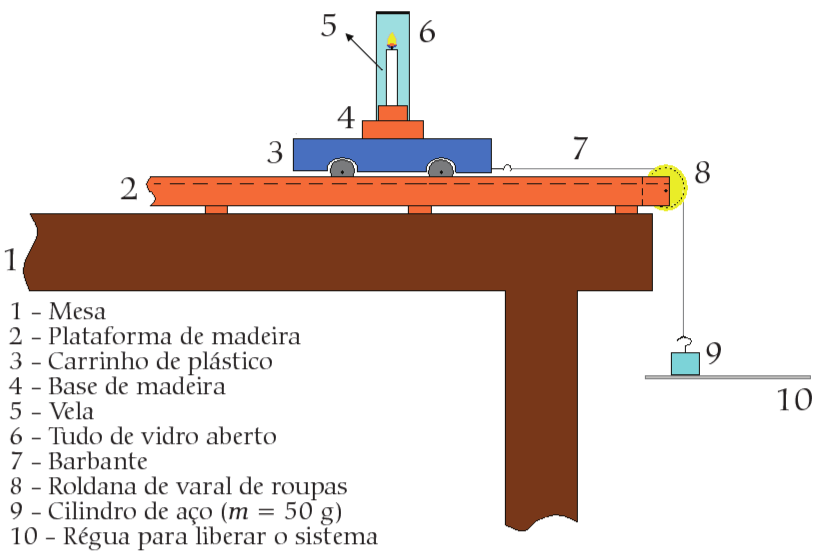
\includegraphics[width=0.65\textwidth]{fig1.png}
  \fonte{\textcite[p. 37]{Souza2010}.}
\end{figure}

Outro exemplo é a ilustração de um pêndulo simples, mostrado na Figura~\ref{fig2} {\color{red}(citar as figuras no texto desta forma)}, em que uma massa \(m\) presa a um fio de comprimento \(l\) oscila em torno de seu ponto de equilíbrio com ângulo \(\theta\) sob a ação da força da gravidade. Note que a legenda da Figura~\ref{fig2} contém basicamente as mesmas informações descritas no parágrafo acima, reforçando a ideia de que uma Figura deve ser independente do texto.

\begin{figure}[ht!]
  \centering
  \caption{Pêndulo simples, mostrando uma massa \(m\) presa a um fio de comprimento \(l\) oscilando com ângulo \(\theta\) em torno do ponto de equilíbrio.}\label{fig2}
  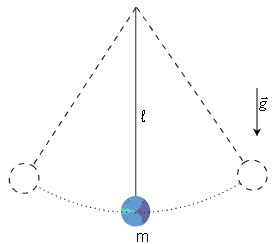
\includegraphics[width=0.4\textwidth]{pendulo.png}
  \fonte{Elaborada pelo autor.}
\end{figure}

\textcolor{red}{\textbf{Observação:} As figuras, tabelas, ilustrações, etc., devem estar juntas com suas legendas e suas fontes na mesma página. A figura não pode ficar em uma página e sua legenda ou fonte em outra.}

Se for necessário incluir alguma foto tirada por vocês mesmos ou uma foto retirada da internet siga o exemplo da Figura~\ref{fig3}.

Quando for necessário discutir ou apresentar equações em qualquer seção do projeto, estas devem ser numeradas e citadas no texto de acordo com o número. Veja o exemplo abaixo:

O período de oscilação \(T\) de um pêndulo simples pode ser calculado através da seguinte expressão:

\begin{equation}\label{periodo}
    T = 2 \pi \sqrt{\dfrac{l}{g}},
\end{equation}
sendo $l$ o comprimento do fio que sustenta a massa $m$ do pêndulo e $g$ a aceleração da gravidade.

\noindent
{\textbf{\color{red}IMPORTANTE:} Todos os parâmetros das equações devem ser explicados no texto, como neste exemplo.}

Se o comprimento $l$ do fio for dado podemos utilizar a Equação~\eqref{periodo} ({\color{red}citar as equações no texto desta forma}) para determinar a aceleração da gravidade através da medida do período de oscilação do pêndulo.

\begin{figure}[ht!]
  \centering
  \caption{Tubo de chama de onda estacionária.}\label{fig3}
  \vspace{1mm}
  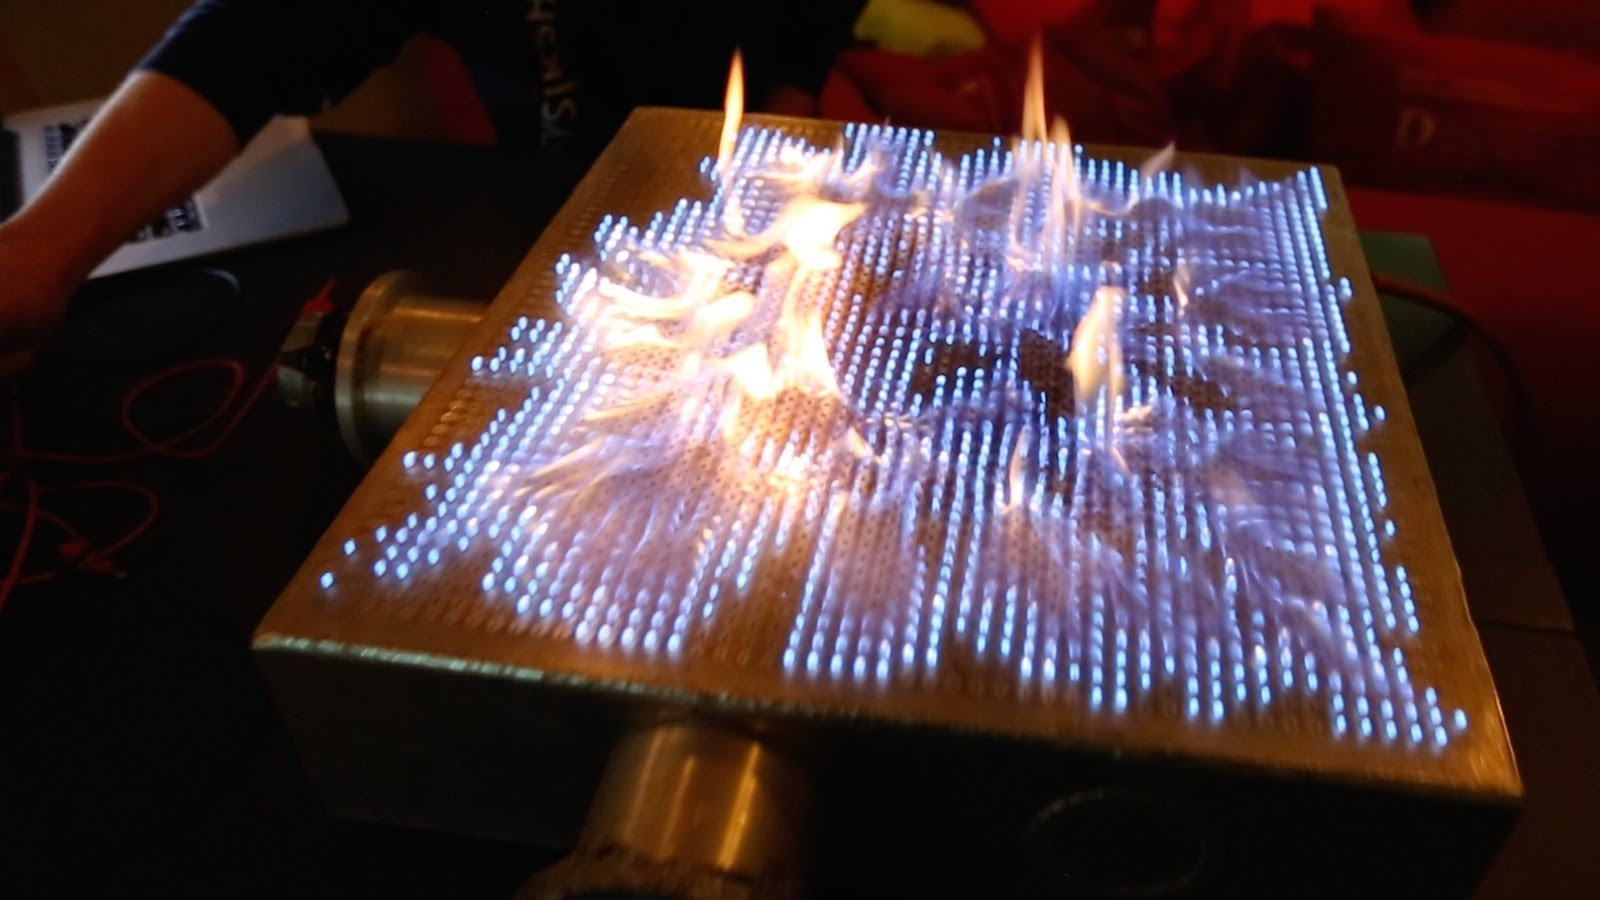
\includegraphics[width=0.6\textwidth]{Chamas.jpg}
  \fonte{JUNIOR, G. \underline{Usando Física para criar um incrível experimento com Fogo e Música.} Disponível em: \url{http://marteeparaosfracos.blogspot.com/2014/04/usando-fisica-para-criar-um-incrivel.html}. Acesso em: 16 nov. 2018.}
\end{figure}

%%%
%%% CRONOGRAMA
%%%
\section{Cronograma de Atividades}

Este tópico é importante para vocês mostrarem aos assessores que avaliarão o projeto, ou no caso para o professor-orientador da disciplina de TCC 1, como vocês pretendem executar a proposta diante do prazo disponível ou determinado. Listem as tarefas que serão executadas em determinado período como pesquisa bibliográfica, busca de materiais para realização do experimento, montagem ou construção do experimento, análise dos resultados obtidos, etc. Esta pode ser feita através de uma tabela. Se caso for necessário incluir outras tabelas na proposta de pesquisa siga o modelo da Tabela~\ref{tabela1} abaixo.

\begin{table}[ht!]
  \centering
  \caption{Cronograma tentativo de atividades.}\label{tabela1}
  \begin{tabular}{cc}
    \toprule
    \textbf{\emph{Período}} & \textbf{\emph{Atividades}}\\
    \midrule
    3 primeiros meses      & Aquisição de materiais para a realização do experimento;        \\
    2º semestre de 2021    & Montagem e testes do experimento;                               \\
    E assim por diante ... & O período pode ser especificado em semanas, meses ou semestres. \\
    \bottomrule
  \end{tabular}
  \fonte{Elaborada pelo autor.}
\end{table}

É importante que o cronograma tentativo apresente de maneira clara o início das atividades, sua execução e a finalização das mesmas, com uma previsão de discussão dos resultados para a escrita da monografia final e a defesa do TCC.

\begin{table}[ht!]
  \begin{center}
    \caption{Cronograma de desenvolvimento do projeto. Cada linha corresponde
      a um objetivo específico da Seção~\ref{sec:objs}. Cada coluna
      corresponde a um mês.}\label{tab:cronog}
    \begin{ganttchart}[hgrid,
                      vgrid,
                      bar/.append style={fill=blue!10,draw=blue},
                      bar top shift=0.1,
                      bar height=0.8,
                      x unit=20mm,
                      y unit chart=6mm]{1}{6}
      \gantttitle{Meses}{6} \\
      \gantttitlelist{1,...,6}{1} \\
      \ganttbar{Seção~\ref{obj1}}{1}{2} \\
      \ganttbar{Seção~\ref{obj2}}{2}{3} \ganttbar{}{5}{6} \\
      \ganttbar{Seção~\ref{obj3}}{4}{6} \\
    \end{ganttchart}
    \fonte{Elaborada pelo autor.}
  \end{center}
\end{table}

% Imprime a bibliografia
\clearpage
\printbibliography[heading=subbibliography]

\end{document}

%%% end of skeleton_tcc_proj.tex
